\question{Спонтанные и индуцированные переходы. Коэффициенты Эйнштейна.}

При индуцированных переходах квантовая система может переводиться из одного 
энергетического состояния в другое \ref{img1.1} как с поглощение энергии 
электромагнитного поля (переход с нижнего на верхний), так и с излучением 
электромагнитной энергии (переход с верхнего на нижний).

\begin{figure}[h!]
	\center
	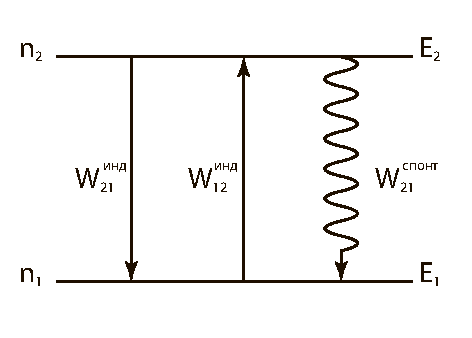
\includegraphics[width=.4\textwidth]{image1_1} \\
	\caption{Схема двух уровней энергии \( E_2 > E_1 \)}
	\label{img1.1}
\end{figure}

Индуцированные переходы обладают следующими важными свойствами.

Во-первых, вероятность индуцированных переходов отлична от нуля только для 
внешнего поля резонансной частоты, энергия которого \( h\nu \) совпадает с 
разностью энергий двух изолированных состояний (\( E_2 \) и \( E_1 \), где 
индекс 2 относится к большей энергии, а 1 -- к меньшей). Это условие 
соответствия постулату Бора:
\[
	h\nu = E_2 - E_1
\]

Во-вторых, кванты электромагнитного поля, излученные при индуцированных 
переходах, полностью тождественны квантам поля, вызвавшего эти переходы. 
То есть внешнее электромагнитное поле и поле, созданное при индуцированных 
переходах, имеют одинаковые частоту, фазу, поляризацию и направление 
распространения -- они тождественны.

В-третьих, вероятность индуцированных переходов в единицу времени 
пропорциональна плотности энергии внешнего поля в единичном спектральном 
интервале:
\[
	W_{12}^\text{инд} = B_{12}\rho_\nu
\]
\[
	W_{21}^\text{инд} = B_{21}\rho_\nu
\]

где \( B_{12} \) и  \( B_{21} \) -- коэффициенты Эйнштейна для индуцированного 
поглощения и излучения соответственно, а порядок индексов 1 и 2 указывает 
направление перехода.

Таким образом индуцированное излучение -- это излучение вынужденное, 
стимулированное внешним излучением. 

Кроме индуцированного внешним полем, существует и самопроизвольное испускание 
излучения. Атомы, находящиеся в верхнем энергетическом состоянии, могут 
совершать спонтанные переходы в нижнее состояние. Эти переходы 
самопроизвольны. Происходящий при спонтанном излучении распад верхнего 
энергетического состояния подобен радиоактивному распаду неустойчивого ядра. 
Вероятность спонтанных переходов не зависит от внешнего электромагнитного 
поля, акты спонтанного излучения никак не связаны с внешним полем. Поэтому 
спонтанное излучение некогерентно по отношению к внешнему полю и играет 
роль собственных шумов. Кроме того, спонтанное излучение опустошает верхний 
энергетический уровень, способствуя возвращению атома в нижнее энергетическое 
состояние.

Спонтанное излучение является эффектом принципиально квантовым, не допускающим 
классической трактовки. В классической механике метастабильное состояние, 
обладающее большей энергией по отношению к некоторому основному устойчивому 
состоянию, в отсутствие внешних возмущений может жить бесконечно долго. В 
квантовой области такое метастабильное состояние спонтанно распадается с 
некоторой отличной от нуля средней скоростью.

Рассмотрим ансамбль квантовых частиц, находящихся в термостате при 
температуре \( T \). Пусть рассматриваемая квантовая система обладает двумя 
уровнями энергии \( E_2 > E_1 \), при переходах между которыми поглощается 
или излучается квант энергии \( h\nu \). При термодинамическом равновесии 
ансамбль не теряет и не приобретает энергии. Следовательно, в единицу времени 
во всём ансамбле общее число переходов из верхнего энергетического состояния 
в нижнее должно быть равным общему числу переходов из нижнего состояние в 
верхнее. Общее число переходов определяется числом частиц на уровнях энергии 
или населенностью уровней. 

При тепловом равновесии распределение частиц по уровням подчиняется формуле 
Больцмана:
\[
	\frac{n_2}{g_2} = \frac{n_1}{g_1}\exp
		\left[ -\frac{E_2 - E_1}{kT}\right]
\]
где \( g_2 \) и \( g_1 \) -- кратность вырождения уровней 2 и 1, 
\( k \) -- постоянная Больцмана.

Полное число переходов \( 2 \rightarrow 1 \) равно произведению числа частиц 
\( n_2 \) в состояние \( 2 \) на вероятность перехода \( 2 \rightarrow 1 \) 
в единицу времени для одной частицы. Вероятность самопроизвольного перехода 
частицы из верхнего состояния в нижнее пропорциональна времени. За время 
\( dt \) эта вероятность составляет по предположению
\[
	dw^\text{спонт} = A_{21} dt
\]
где \( A_{21} \) -- коэффициент Эйнштейна для спонтанного излучения. Таким 
образом вероятность спонтанного испускания излучения в единицу времени 
постоянна и равна по определению соответствующему коэффициенту Эйнштейна 
\( A_{21} \):
\[
	W_{21}^\text{спонт} = A_{21}
\]

Частицы рассматриваемого ансамбля находятся в поле их собственного излучения, 
плотность энергии которого в единичном спектральном интервале составляет 
\( \rho_\nu \). Это поле индуцирует переходы из верхнего состояния в нижнее 
и обратно. Вероятности этих переходов пропорциональны \( \rho_\nu \). 
Комбинируя предыдущие формулы, можем из условия равновесия
\[
	g_1 B_{12} \rho_\nu \exp\left[ -\frac{E_1}{kT} \right] = 
	g_2 \left( B_{21}\rho_nu + A_{21} \right)
		\exp\left[ -\frac{E_2}{kT} \right]
\]
найти соотношения между коэффициентами \( A_{21}, B_{12}, B_{21} \). Это 
уравнение позволяет легко найти плотность энергии поля излучения 
рассматриваемой равновесной квантовой системы:
\[
	\rho_\nu = \frac{A_{21}}{B_{21}}
		\left[ 
			\frac{g_1 B_{12}}{g_2 B_{21}}\exp\frac{E_2 - E_1}{kT} - 1 
		\right]^{-1}
\]

Эйнштейн постулировал, что излучение, испускаемое и поглощаемое при 
равновесных переходах между энергетическими состояниями рассматриваемой 
равновесной квантовой системы, описывается формулой Планка для 
равновесного излучения абсолютно чёрного тела. Тогда для свободного 
пространства
\[
	\rho_\nu = \frac{8\pi\nu^2}{c^3}\frac{h\nu}{\exp[h\nu/kT] - 1}
\]
где \( c \) -- скорость света.

Если сопоставить две эти формулы с условием Бора, то получим что 
постулат Эйнштейна совместим с постулатом Бора. Дальнейшее сравнение приведёт 
к выводу:
\[
	g_1 B_{12} = g_2 B_{21}
\]

Это соотношение говорит о равновероятности индуцированных излучения и 
поглощения. Далее, вероятность спонтанного излучения пропорциональна 
коэффициенту Эйнштейна для индуцированного излучения:
\[
	A_{21} = \frac{8\pi\nu^2}{c^3}h\nu B_{21}
\]

Таким образом, для описания термодинамического равновесия между системой 
квантовых частиц и полем её излучения Эйнштейн ввёл индуцированные полем 
равновероятные переходы из верхнего состояния в нижнее и из нижнего в верхнее. 
Требование равновесия приводит к такому соотношению между спонтанными и 
индуцированным излучениями, при котором для одной частицы вероятность 
переходов в единицу времени с испусканием квантов излучения равна
\[
	W^\text{изл} = \left( \frac{8\pi\nu^2}{c^3} + \rho_\nu \right)B_{21}
\]